\section{Bundle Adjustment}\label{sec:bundle-adjustment}

At the end of the previous chapter we asked how NLLS can be used for the \textbf{3D reconstruction} with cameras. The answer is \textbf{bundle adjustment} (BA). In this chapter we write it as a least squares problem, we see why its Jacobian is very sparse, and how this sparsity is exploited (Schur trick). Finally, we generalize BA to \textbf{factor graph optimization}, which is the common framework behind visual odometry, SLAM and sensor fusion.

\subsection{What is bundle adjustment}
\textbf{Bundle adjustment} means optimizing at the same time the \textbf{camera parameters} (intrinsics and extrinsics) and the \textbf{3D landmarks}, using the images.

The name comes from the \textbf{bundles of light rays}. Each 3D point emits rays that are projected onto the image planes of several cameras, where they are detected as feature points. The goal of the optimization is to \emph{adjust} the camera poses and the 3D points so that the projected 2D points (the bundles) match the detected features as closely as possible.

\begin{figure}[H]
    \centering
    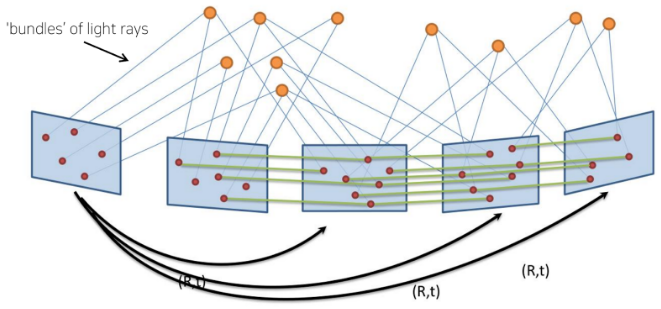
\includegraphics[width=0.65\textwidth]{images/C10_1.png}
    \caption{Bundles of light rays: each 3D point (orange) is observed by several cameras, related by their poses $(R,t)$}
\end{figure}

\subsection{Mathematical formulation}
BA is an NLLS problem that minimizes the \textbf{reprojection error}, i.e.\ the distance between the observed 2D point and the projection of the estimated 3D point:
\[
\min_{\{R_i,\, t_i,\, K,\, d,\, X_j\}} \ \sum_{i,j} \left\| x_{ij} - \pi\!\left(R_i, t_i, K, d, X_j\right) \right\|_2^2
\]
where:
\begin{compactitemize}
    \item $R_i, t_i$ are the rotation and translation of the $i$-th camera;
    \item $K$ are the camera intrinsics;
    \item $d$ are the distortion parameters;
    \item $X_j$ is the $j$-th 3D point;
    \item $x_{ij}$ is the observed 2D point $j$ in image $i$;
    \item $\pi(\cdot)$ is the projection function.
\end{compactitemize}
If the camera is already calibrated, optimizing also $K$ and $d$ is optional, and they can be kept fixed.

The rotations $R_i$ live in $SO(3)$, so in practice they are updated with the exponential map seen in the previous chapter ($R_i \boxplus \xi_i$), and not with a simple sum.

\subsubsection{Reminder: the projection function}
The projection function $\pi$ is the camera model of Section~\ref{chap:cameras}, applied in three steps:
\begin{enumerate}
    \item \textbf{extrinsics}: the world point $p$ is moved into the camera frame and normalized by its depth:
    \[
    P' = R\,p + t, \qquad P_c = \left[\, P'_X / P'_Z,\ P'_Y / P'_Z,\ 1 \,\right]^T
    \]
    \item \textbf{distortion}: the radial distortion is applied to the normalized coordinates:
    \[
    u'_c = u_c \left(1 + k_1 r_c^2 + k_2 r_c^4\right), \qquad v'_c = v_c \left(1 + k_1 r_c^2 + k_2 r_c^4\right)
    \]
    \item \textbf{intrinsics}: the point is converted to pixel coordinates:
    \[
    u_s = f_x\, u'_c + c_x, \qquad v_s = f_y\, v'_c + c_y
    \]
\end{enumerate}

\begin{figure}[H]
    \centering
    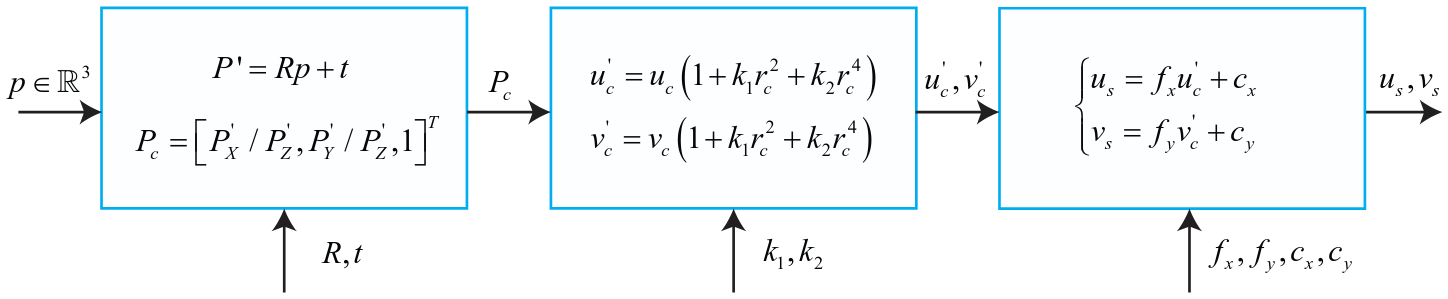
\includegraphics[width=0.95\textwidth]{images/C10_2.png}
    \caption{Projection function: extrinsics $(R,t)$, distortion $(k_1,k_2)$ and intrinsics $(f_x,f_y,c_x,c_y)$}
\end{figure}

\subsection{Jacobian sparsity}
The Jacobian and the Hessian of bundle adjustment are \textbf{highly sparse}, for three reasons:
\begin{compactitemize}
    \item if a point is not visible in a camera, there is \textbf{no residual} for that pair;
    \item two camera poses never appear in the same residual, so each row of $J$ contains the gradient with respect to \textbf{only one pose};
    \item two 3D points never appear in the same residual, so each row of $J$ contains the gradient with respect to \textbf{only one point}.
\end{compactitemize}
Each row of $J$ has therefore only two non-zero blocks: one for the pose and one for the point of that observation.

This is the typical situation whenever we estimate a \textbf{trajectory}, i.e.\ a sequence of poses (roto-translations) that changes over time. The index $i$ of the poses is exactly the \textbf{time index} of the parameters: $R_i, t_i$ is the pose of the camera (or of the vehicle) at time step $i$. Each residual only involves the parameters of one instant, or of two consecutive instants as for odometry (Section~\ref{sec:factor-graph}). Its derivatives with respect to all the other poses are therefore zero. As a consequence, most entries of the Jacobian are \textbf{zero}, and the longer the trajectory, the sparser the problem becomes.

Consider a small problem with only two camera poses $C_1$ and $C_2$, where the points $P_1, P_2, P_3, P_4$ are visible in $C_1$ and the points $P_3, P_4, P_5, P_6$ are visible in $C_2$. We get 8 residuals $e_{ij}$, and the row $J_{ij}$ is non-zero only in the columns of $C_i$ and $P_j$. The Hessian (in its Gauss--Newton approximation)
\[
H = J^T J
\]
inherits this structure. A block $H_{ab}$ is non-zero only if the variables $a$ and $b$ appear together in at least one residual.

\begin{figure}[H]
    \centering
    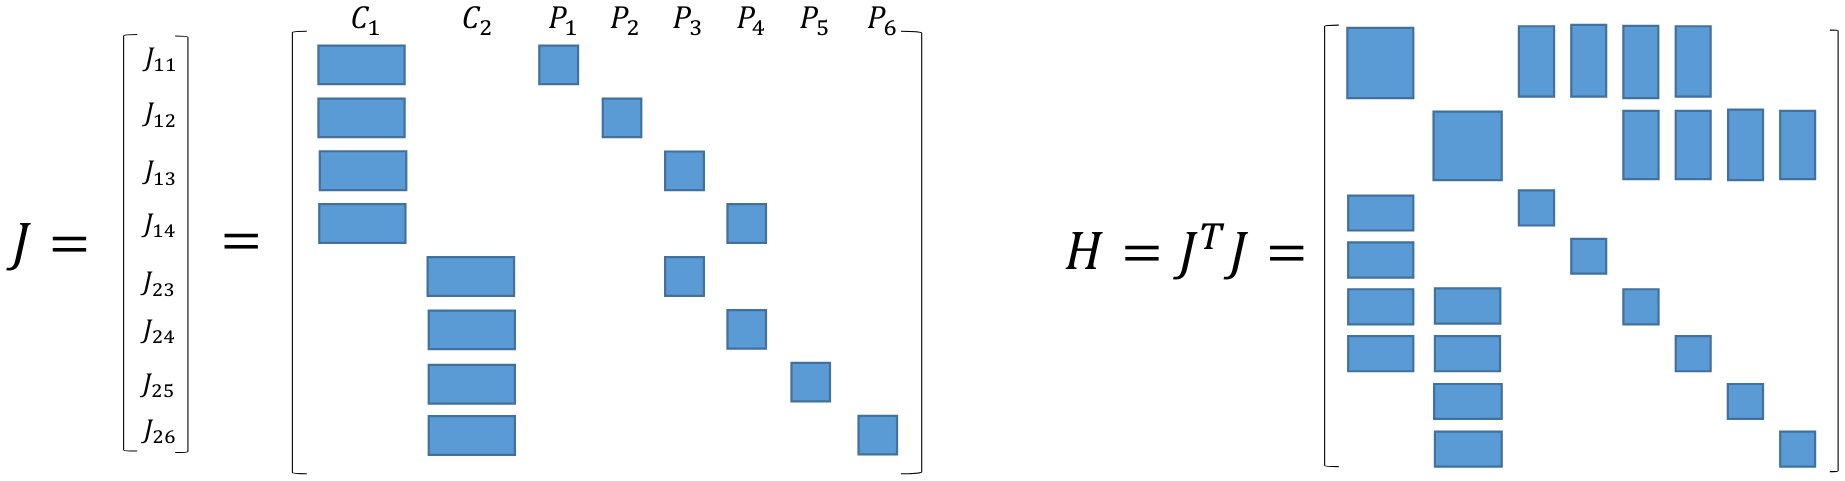
\includegraphics[width=0.95\textwidth]{images/C10_3.png}
    \caption{Structure of $J$ and $H=J^TJ$ for 2 cameras and 6 points (blue = non-zero block)}
\end{figure}

\subsection{Exploiting the sparsity of the Hessian}
In a real BA problem the Hessian is very sparse and has a special structure, called the \textbf{``pickaxe'' matrix} (or arrowhead matrix), because of its shape. We order the variables with the camera poses first and the 3D points after. Then $H$ has:
\begin{compactitemize}
    \item a small block at the top left for the cameras;
    \item a long \textbf{block diagonal} for the points;
    \item two sparse off-diagonal bands, which link the cameras with the points they observe.
\end{compactitemize}
We can exploit this structure to solve the linear system of each iteration efficiently:
\[
H\, \Delta x = g
\]

\begin{figure}[H]
    \centering
    \begin{subfigure}[b]{0.42\textwidth}
        \centering
        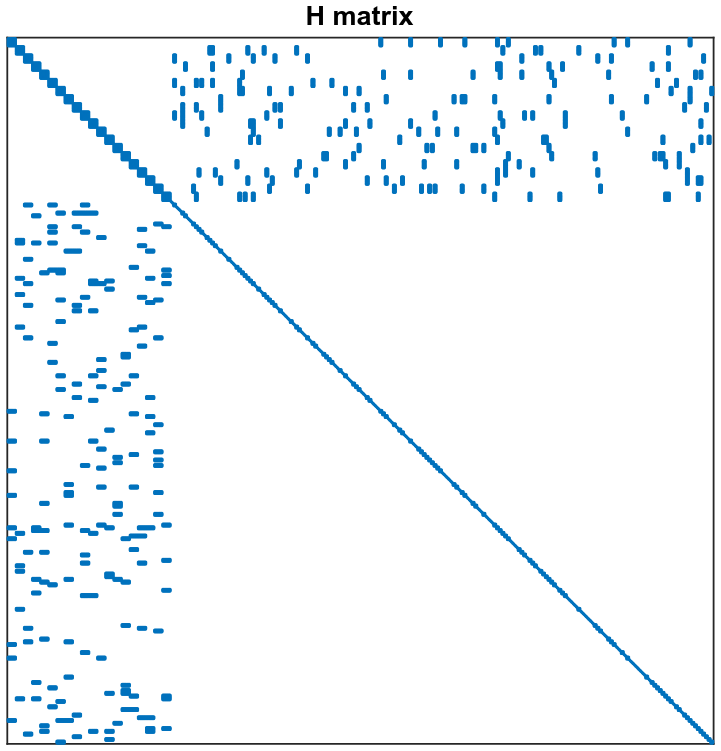
\includegraphics[height=5.5cm]{images/C10_4.png}
        \caption{Sparsity pattern of a real BA Hessian}
    \end{subfigure}
    \hfill
    \begin{subfigure}[b]{0.42\textwidth}
        \centering
        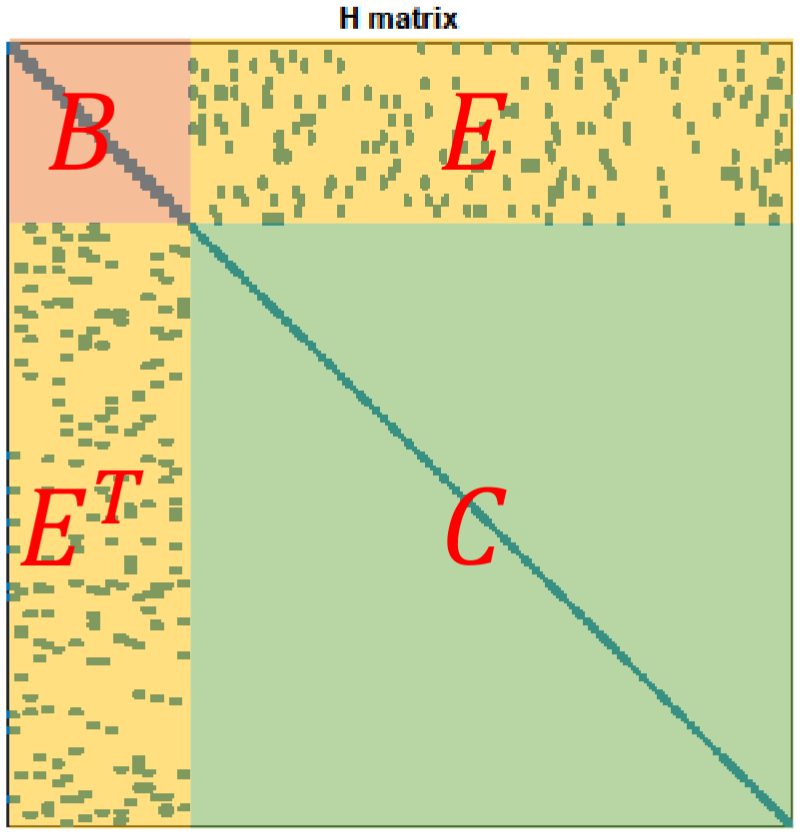
\includegraphics[height=5.5cm]{images/C10_5.png}
        \caption{Block structure: $B$, $E$, $E^T$, $C$}
    \end{subfigure}
    \caption{The ``pickaxe'' structure of the BA Hessian}
\end{figure}

\subsection{Schur trick}
We split the unknowns into the camera part $\Delta x_c$ and the point part $\Delta x_p$. The system $H\,\Delta x = g$ can then be written in blocks:
\[
\begin{bmatrix} B & E \\ E^T & C \end{bmatrix}
\begin{bmatrix} \Delta x_c \\ \Delta x_p \end{bmatrix}
=
\begin{bmatrix} g_c \\ g_p \end{bmatrix}
\]
where:
\begin{compactitemize}
    \item $B$ is a \textbf{block diagonal} matrix for the camera poses (one block per pose), and its size equals the number of poses;
    \item $C$ is a \textbf{block diagonal} matrix with $3\times 3$ blocks (one block per 3D point), and its total size equals the number of points;
    \item $E$ contains the mixed camera--point terms.
\end{compactitemize}

The number of points is usually \textbf{much larger} than the number of camera variables, so $C$ is much bigger than $B$. However, inverting a block diagonal matrix is much easier than inverting a general matrix: we only need to invert each diagonal block separately. For $C$ this means inverting many small $3\times 3$ matrices, which has a cost that is only \emph{linear} in the number of points:
\[
C^{-1} = \operatorname{diag}\!\left(C_1^{-1}, C_2^{-1}, \dots, C_{N_p}^{-1}\right)
\]

The Schur trick eliminates $\Delta x_p$ with a \textbf{Gaussian elimination by blocks}. We multiply both sides on the left by the matrix
\[
\begin{bmatrix} I & -E C^{-1} \\ 0 & I \end{bmatrix}
\]
which gives:
\[
\begin{bmatrix} I & -E C^{-1} \\ 0 & I \end{bmatrix}
\begin{bmatrix} B & E \\ E^T & C \end{bmatrix}
\begin{bmatrix} \Delta x_c \\ \Delta x_p \end{bmatrix}
=
\begin{bmatrix} I & -E C^{-1} \\ 0 & I \end{bmatrix}
\begin{bmatrix} g_c \\ g_p \end{bmatrix}
\]
Computing the products row by row:
\begin{compactitemize}
    \item first row, first block: $B - E C^{-1} E^T$;
    \item first row, second block: $E - E C^{-1} C = E - E = 0$;
    \item first row, right-hand side: $g_c - E C^{-1} g_p$;
    \item the second row is unchanged.
\end{compactitemize}
So the system becomes:
\[
\begin{bmatrix} B - E C^{-1} E^T & 0 \\ E^T & C \end{bmatrix}
\begin{bmatrix} \Delta x_c \\ \Delta x_p \end{bmatrix}
=
\begin{bmatrix} g_c - E C^{-1} g_p \\ g_p \end{bmatrix}
\]
The first row no longer depends on $\Delta x_p$. The Schur trick then solves the problem in two steps.

\textbf{Step 1.} We solve the \textbf{reduced camera system}:
\[
\left(B - E C^{-1} E^T\right) \Delta x_c = g_c - E C^{-1} g_p
\]
This system has the same dimension as $B$, so it is small, and it is still sparse. The matrix $B - E C^{-1} E^T$ is called the \textbf{Schur complement} of $C$ in $H$.

\textbf{Step 2.} We substitute the computed $\Delta x_c$ back into the second row, $E^T \Delta x_c + C\, \Delta x_p = g_p$, and get the points:
\[
\Delta x_p = C^{-1} \left(g_p - E^T \Delta x_c\right)
\]

In both steps we only need $C^{-1}$, which is easy to compute because $C$ is block diagonal. So instead of factorizing the whole huge matrix $H$, we factorize only the small reduced system for the cameras. The points are then recovered one by one, independently.

\subsection{Hessian interpretation}
The Hessian matrix can be seen as the \textbf{adjacency matrix of a graph}:
\begin{compactitemize}
    \item the \textbf{nodes} of the graph are the variables to estimate (camera poses and 3D points);
    \item an \textbf{arc} connects two variables that appear in the same residual.
\end{compactitemize}
For example, the residual $e_{26}$ (point $P_6$ observed by camera $C_2$) creates the non-zero block in row $C_2$ and column $P_6$ of $H$, and the arc between the nodes $C_2$ and $P_6$ in the graph. The sparsity of the graph is therefore directly connected to the sparsity of the problem: few arcs means a sparse Hessian.

\begin{figure}[H]
    \centering
    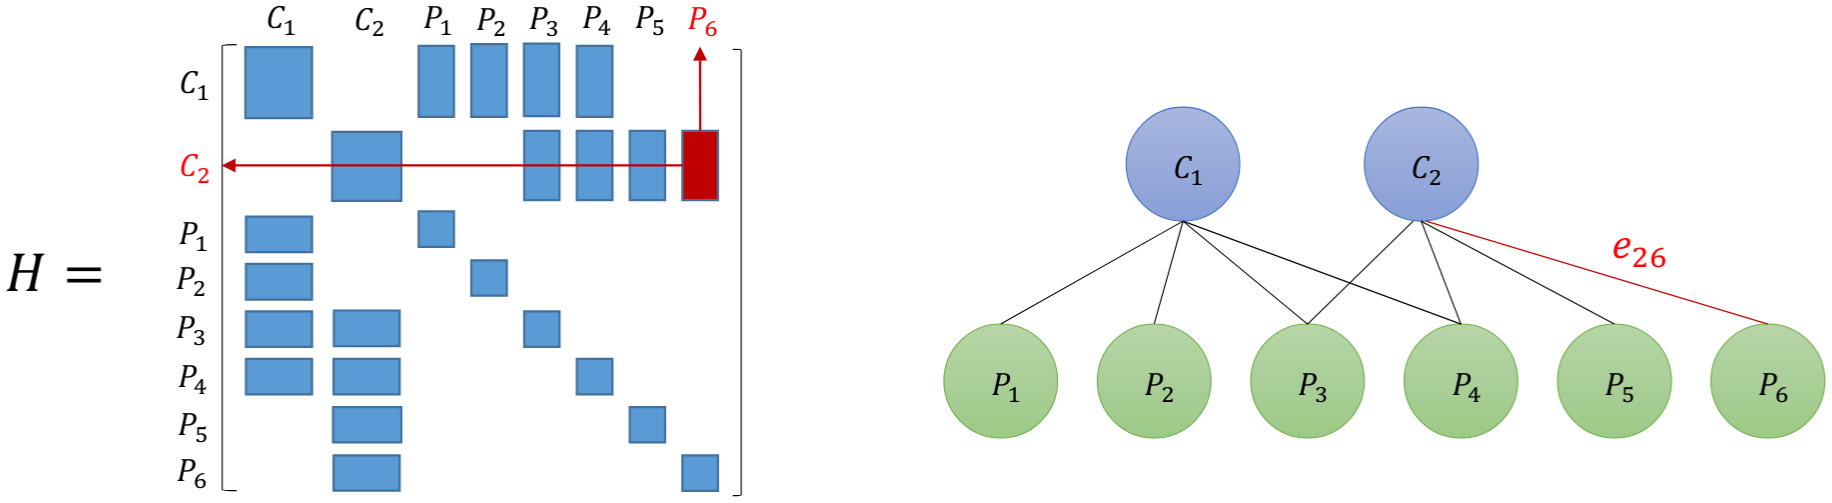
\includegraphics[width=0.95\textwidth]{images/C10_6.png}
    \caption{The Hessian as the adjacency matrix of a graph: the residual $e_{26}$ corresponds to the block $(C_2, P_6)$ and to the arc $C_2$--$P_6$}
\end{figure}

\subsection{Factor graph optimization}\label{sec:factor-graph}
BA is a special case of \textbf{factor graph optimization}. In general, any NLLS problem can be represented in graph form:
\begin{compactitemize}
    \item the variables to optimize are called \textbf{states} (circles in the figures);
    \item the residuals are called \textbf{factors} (small squares). A factor can involve from 1 to $N$ states, and it is connected to all the states it depends on.
\end{compactitemize}
The cost to minimize is the sum of all the factors. Adding a new sensor simply means adding a new type of factor to the graph, so this representation is a very flexible way to fuse different measurements.

\subsubsection{Example: Visual-Inertial Odometry (VIO)}
In VIO:
\begin{compactitemize}
    \item the states $x_i$ are the camera poses;
    \item the states $l_j$ are the 3D landmark positions;
    \item the \textbf{black factors} are the 2D reprojection residuals, which connect a pose to a landmark;
    \item the \textbf{green factors} are the odometry measurements from the IMU or other sensors. They define the relative motion (delta position and rotation) between two consecutive states.
\end{compactitemize}
The cost is:
\[
\min_{\{T_i,\, l_j\}} \ \sum_{i,j} \left\| x_{ij} - \pi\!\left(T_i, K, d, l_j\right) \right\|_2^2 \;+\; \sum_{i} \left\| o_i - T_i^{-1} T_{i+1} \right\|_2^2
\]
where $T_i$ is the pose of the $i$-th camera, $x_{ij}$ the observation of landmark $l_j$ in frame $i$, and $o_i$ the relative motion between frames $i$ and $i+1$ measured by odometry. The term $T_i^{-1}T_{i+1}$ is the relative pose predicted by the states.

\begin{figure}[H]
    \centering
    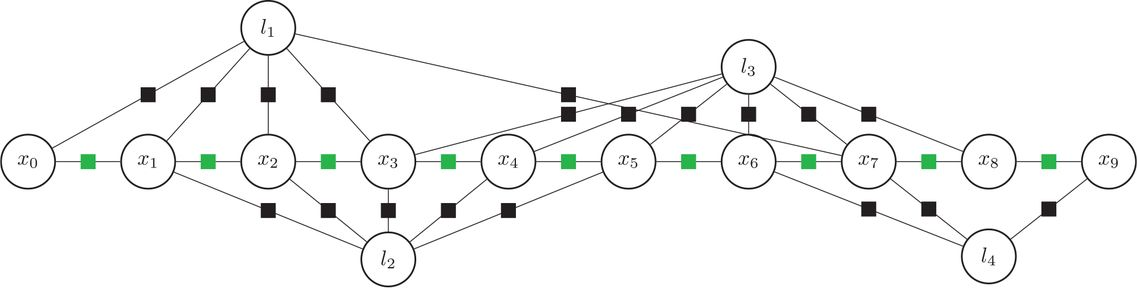
\includegraphics[width=0.9\textwidth]{images/C10_7.png}
    \caption{Factor graph of VIO: poses $x_i$, landmarks $l_j$, reprojection factors (black) and odometry factors (green)}
\end{figure}

\subsubsection{Example: Inertial Navigation System (INS)}
In an INS there are no landmarks:
\begin{compactitemize}
    \item the states $x_i$ are the vehicle poses;
    \item the \textbf{green and blue factors} are odometry measurements from the IMU and other sensors (e.g.\ wheel odometry), and each one defines the relative motion between two consecutive states;
    \item the \textbf{black factors} are sporadic GPS positions, and each one is connected to a single state.
\end{compactitemize}
The cost is:
\[
\min_{\{T_i\}} \ \sum_{ij} \left\| o_{ij} - T_i^{-1} T_{i+1} \right\|_2^2 \;+\; \sum_{i} \left\| g_i - t_i \right\|_2^2
\]
where $o_{ij}$ is the relative motion measured by the $j$-th odometry sensor between the states $i$ and $i+1$, $g_i$ the GPS position and $t_i$ the translation part of the pose $T_i$. The slide writes $\{T_i, l_j\}$ under the $\min$, but there are no landmarks here, so only the poses are optimized.

Odometry alone drifts over time, while GPS is absolute but sporadic and noisy. The factor graph fuses the two: the GPS factors ``anchor'' the trajectory, and the odometry factors keep it smooth between two GPS fixes.

\begin{figure}[H]
    \centering
    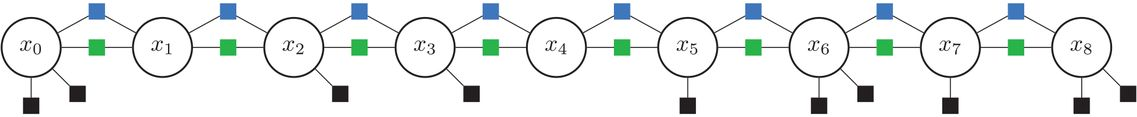
\includegraphics[width=0.9\textwidth]{images/C10_8.png}
    \caption{Factor graph of an INS: odometry factors (green and blue) and sporadic GPS factors (black)}
\end{figure}

\subsubsection{Other examples}
The same framework covers many other problems.

\textbf{Localization in a known map.} Here the black factors are \textbf{known landmarks} from a map. Their positions are not states, because they are already known, so each factor is connected only to the pose that observes it.

\textbf{Multi-model with online weighting.} Additional states $w_i$ represent the weights of the different measurement models. They are estimated together with the poses $x_i$, so the importance of each model is adapted online. The yellow factors act on the weights only.

\begin{figure}[H]
    \centering
    \begin{subfigure}[b]{\textwidth}
        \centering
        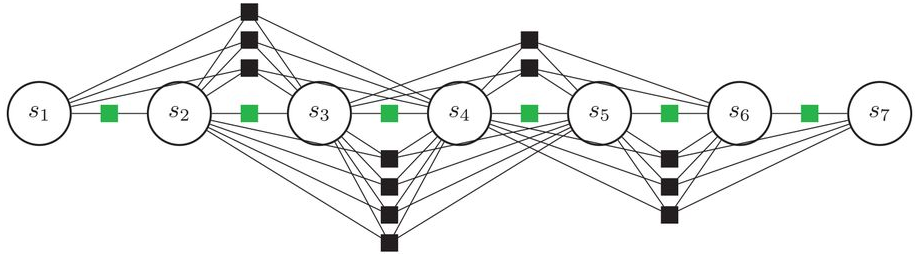
\includegraphics[width=0.7\textwidth]{images/C10_9.png}
        \caption{Localization with known landmarks from a map (black)}
    \end{subfigure}

    \vspace{0.4cm}
    \begin{subfigure}[b]{\textwidth}
        \centering
        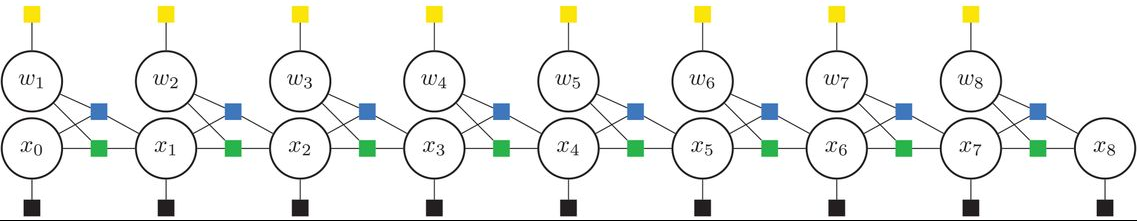
\includegraphics[width=0.85\textwidth]{images/C10_10.png}
        \caption{Multi-model with online weighting}
    \end{subfigure}
    \caption{Other examples of factor graphs}
\end{figure}

\subsection{Extensions of BA}
BA is ``just'' a building block for more complex methods:
\begin{compactitemize}
    \item \textbf{Visual-Inertial Odometry (VIO)}: it integrates the IMU or other sensors to \textbf{recover the scale}, which a single camera cannot observe, and it optimizes over a \textbf{sliding window} of recent frames, so the cost stays bounded;
    \item \textbf{Visual SLAM (VSLAM)}: like VIO, but it also builds an internal \textbf{map}, which it uses to re-localize when it passes again in the same spot (loop closure).
\end{compactitemize}

\subsection{Research on 3D reconstruction}
Besides the classical geometric pipeline, current research uses learning-based methods:
\begin{compactitemize}
    \item \textbf{Neural Radiance Fields (NeRFs)}:
    \begin{compactitemize}
        \item they reconstruct unseen views of a scene from a few images;
        \item they learn a continuous volumetric representation of the scene;
        \item newer versions are much faster in training and inference (e.g.\ Instant-NGP, Zip-NeRF, Nerfacto).
    \end{compactitemize}
    \item \textbf{Gaussian Splatting}: it represents the scene with 3D Gaussians instead of voxels or meshes, which allows real-time rendering with high visual quality.
    \item \textbf{VGGT}: a feed-forward network that directly estimates camera poses, depth maps, 3D points and tracks, without an iterative optimization.
\end{compactitemize}
